\documentclass[tikz,border=12pt]{standalone}
\usepackage{tikz}
\usetikzlibrary{positioning, arrows.meta, calc}

\definecolor{prose}{RGB}{70, 130, 180}
\definecolor{html}{RGB}{60, 179, 113}
\definecolor{code}{RGB}{218, 165, 32}
\definecolor{md}{RGB}{200, 110, 110}
\definecolor{json}{RGB}{178, 102, 178}
\definecolor{yaml}{RGB}{120, 130, 160}

\begin{document}
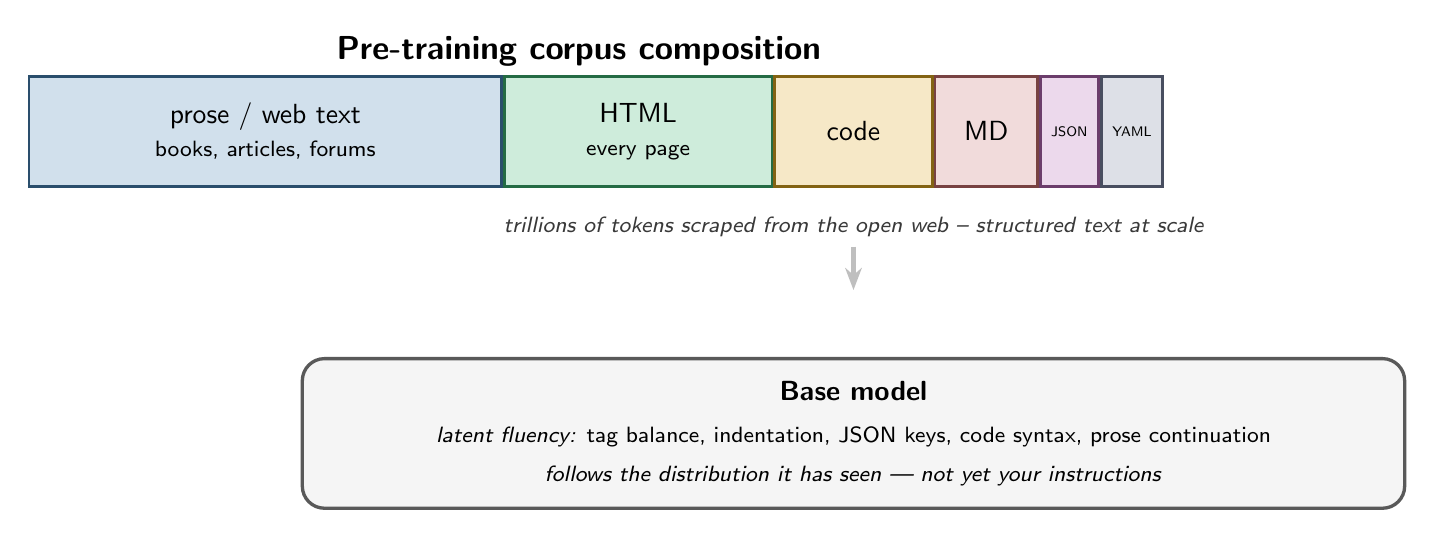
\begin{tikzpicture}[
    slab/.style={
        rectangle, fill=#1!25, draw=#1!60!black,
        minimum height=1.4cm, line width=1pt,
        font=\sffamily, align=center,
        inner sep=4pt,
    },
    bigarrow/.style={-{Stealth[length=8pt]}, line width=1.8pt, draw=gray!50},
    model/.style={
        rectangle, rounded corners=8pt, draw=gray!70!black, fill=gray!8,
        line width=1.2pt, minimum width=14cm, minimum height=1.9cm,
        font=\sffamily, align=center,
    },
]

% --- Title ---
\node[font=\sffamily\large\bfseries] (title) at (0,0)
    {Pre-training corpus composition};

% --- Slab row, total width = 14cm, anchored under title ---
\coordinate (rowstart) at ($(title.south)+(-7cm,-0.7cm)$);
\node[slab=prose, minimum width=6cm, anchor=west] (prose) at (rowstart)
    {prose / web text\\\footnotesize books, articles, forums};
\node[slab=html,  minimum width=3.4cm, anchor=west] (html)  at (prose.east)
    {HTML\\\footnotesize every page};
\node[slab=code,  minimum width=2.0cm, anchor=west] (code)  at (html.east)
    {code};
\node[slab=md,    minimum width=1.3cm, anchor=west] (md)    at (code.east)
    {MD};
\node[slab=json,  minimum width=0.7cm, anchor=west] (json)  at (md.east)
    {\tiny JSON};
\node[slab=yaml,  minimum width=0.6cm, anchor=west] (yaml)  at (json.east)
    {\tiny YAML};

% --- Caption under slab row ---
\node[font=\sffamily\footnotesize\itshape, text=gray!45!black,
      below=0.25cm of code] (cap)
    {trillions of tokens scraped from the open web -- structured text at scale};

% --- Arrow to base model ---
\draw[bigarrow] (cap.south) -- ++(0,-0.55);

% --- Base model ---
\node[model, below=1.4cm of cap] (model) {
    \textbf{Base model}\\[3pt]
    \footnotesize\textit{latent fluency:} tag balance, indentation, JSON keys,
    code syntax, prose continuation\\[2pt]
    \footnotesize\textit{follows the distribution it has seen ---
    not yet your instructions}
};

\end{tikzpicture}
\end{document}
